% Shared preamble for the English summaries in this repository.
\documentclass[11pt,a4paper]{article}
\usepackage[margin=2.2cm]{geometry}
\usepackage[T1]{fontenc}
\usepackage[utf8]{inputenc}
\usepackage{lmodern}
\usepackage{amsmath,amssymb}
\usepackage{graphicx}
\usepackage{booktabs}
\usepackage{enumitem}
\usepackage[hidelinks]{hyperref}
\setlist{itemsep=2pt,topsep=4pt}
\setlength{\parindent}{0pt}
\setlength{\parskip}{5pt}
\graphicspath{{figures/}}
\newcommand{\summaryheader}[3]{%
  \begin{center}
    {\Large\bfseries #2}\\[3pt]
    {\large #1}\\[3pt]
    {\small Arshia Goshtasbi \textbullet{} MSc Electrical Engineering (Control), Iran University of Science and Technology \textbullet{} #3}
  \end{center}
  \vspace{2pt}\hrule\vspace{8pt}\par}

\begin{document}
\summaryheader{Machine Learning, Course Project}{Solving a Sudoku from a Photo: Rectification, Grid Detection, Digit CNN and Backtracking}{Spring 1404 (2025)}

\textbf{Goal.} Take a phone photo of a printed Sudoku and return the solved puzzle drawn on the image. The project was handed in in four phases; all of them are in \texttt{sudoku.ipynb} (and the exported \texttt{sudoku.py}).

\begin{description}
  \item[Phase 1: rectify the paper.] Grayscale, Gaussian blur, Canny edges and dilation. The largest external contour is taken as the sheet and approximated by a quadrilateral (or the minimum-area rectangle if the approximation does not have four corners). The corners are ordered and a perspective warp gives a front view of the paper.
  \item[Phase 2: find the grid.] Adaptive thresholding of the rectified sheet, then the largest convex four-sided contour with an aspect ratio between 0.8 and 1.2.
  \item[Phase 3: read the digits.] The grid's bounding box is split into $9\times9$ cells (2-pixel inner padding). A cell whose mean intensity is above 240 counts as empty. Otherwise the largest contour in the Otsu-thresholded cell is cropped, scaled to fit $25\times25$ and centred on a $28\times28$ canvas. Two Keras CNNs were trained on the Kaggle \emph{printed digits} dataset (80/20 split):
  \begin{itemize}
    \item a simple model: two convolution and pooling blocks and a 64-unit dense layer;
    \item an improved model: three convolution blocks with batch normalisation and dropout, global average pooling, and training with augmentation (zoom and shift $\pm10\%$, contrast $\pm20\%$), early stopping and learning-rate reduction.
  \end{itemize}
  A prediction is only accepted if its softmax confidence is above $0.8$.
  \item[Phase 4: solve and draw.] Depth-first backtracking that checks rows, columns and $3\times3$ boxes; the missing digits are written on the rectified image in red.
\end{description}

\textbf{What I re-checked for this repository.} The original test photos came with the course and are not included. TensorFlow has no conda-forge build for Windows, so I wrote \texttt{keras\_numpy.py}, a NumPy forward pass that reads the saved \texttt{.h5} models; \texttt{run\_demo.py} runs the four phases unchanged from \texttt{sudoku.py} with it.
\begin{itemize}
  \item \emph{Classifiers} (\texttt{evaluate\_models.py}): on all 6299 images of the digits dataset, training images included (the exact Keras split can't be rebuilt without TensorFlow), the simple model scores $98.8\%$ and the improved one $97.4\%$. The improved model's weakest class is ``1'' ($86.7\%$).
  \item \emph{Pipeline} (\texttt{make\_test\_photos.py} renders three synthetic photos with a random perspective, rotation, shading, blur and noise; Figure~\ref{fig:demo}): rectification and cell segmentation work on all three. No digit was misread and no empty cell was read as a digit, but many clues were missed: 14 of 35, 15 of 32 and 1 of 28. In the missed cells a piece of grid line is left inside the crop and is the largest contour, so the classifier sees a line, not the digit. With clues missing, backtracking still finds a valid grid, but not the one that matches the printed puzzle. A tighter crop or removing lines before the contour step would fix this; I left the course code as it was.
\end{itemize}

\begin{figure}[h]\centering
  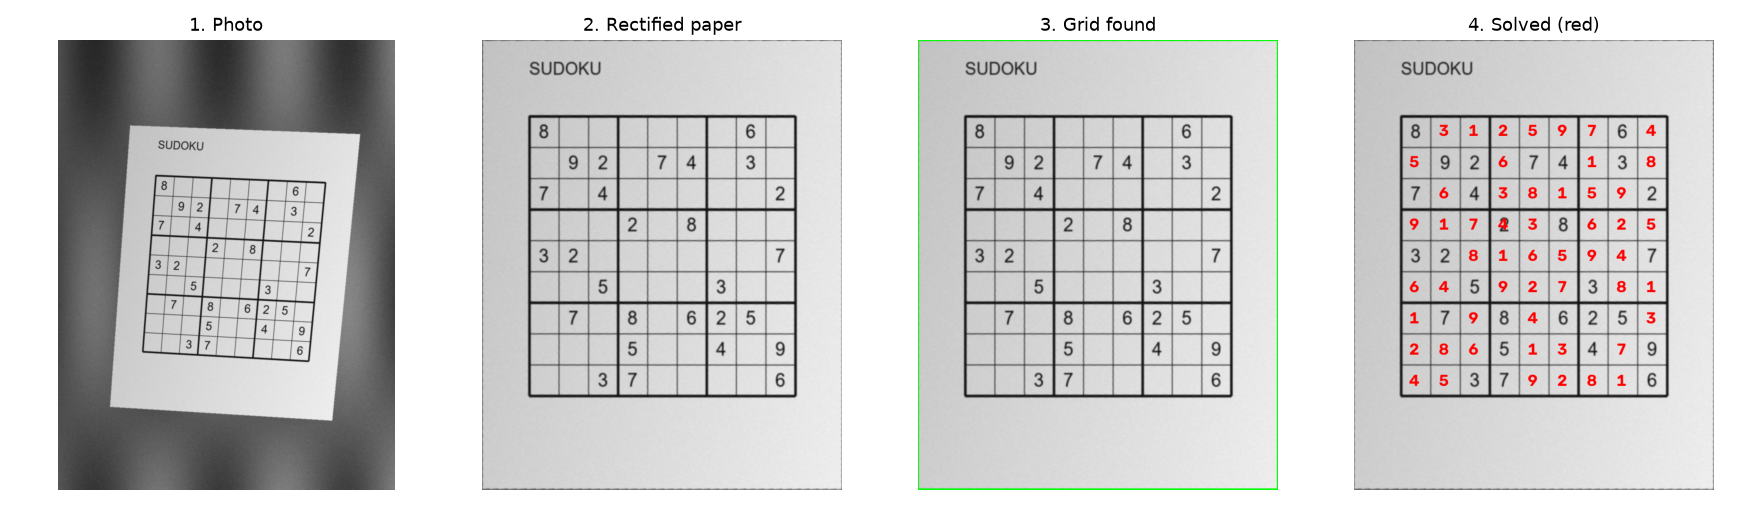
\includegraphics[width=\linewidth]{synthetic_3_pipeline.png}
  \caption{Synthetic photo 3: input, rectified sheet, the Phase 2 outline (here it found the sheet border, not the grid), and the filled-in grid. 27 of 28 clues were read; the 2 in row 4, column 4 was missed, so the completion is a valid grid but not the intended one.}\label{fig:demo}
\end{figure}
\end{document}
